\documentclass{VUMIFPSkursinis}
\usepackage{algorithmicx}
\usepackage{algorithm}
\usepackage{algpseudocode}
\usepackage{amsfonts}
\usepackage{amsmath}
\usepackage{bm}
\usepackage{caption}
\usepackage{color}
\usepackage{float}
\usepackage{graphicx}
\usepackage{enumitem}
\usepackage{listings}
\usepackage{subfig}
\usepackage{array}
\usepackage{wrapfig}
\usepackage{booktabs}
\usepackage{longtable}
\usepackage{eurosym}
\usepackage[hidelinks]{hyperref}
\usepackage{todonotes}
\usepackage[utf8]{inputenc}

\definecolor{dkgreen}{rgb}{0,0.6,0}
\definecolor{gray}{rgb}{0.5,0.5,0.5}
\definecolor{mauve}{rgb}{0.58,0,0.82}

% \lstdefinelanguage{Agda}{%
% language=Haskell
% }

\lstset{
  language=Haskell,
  aboveskip=3mm,
  belowskip=3mm,
  showstringspaces=false,
	columns=flexible,
	deletekeywords=[2]{zero, sum, tail},
	deletekeywords={zero, sum, tail},
  basicstyle={\small\ttfamily},
  numbers=none,
  numberstyle=\tiny\color{gray},
  keywordstyle=\color{blue},
  commentstyle=\color{dkgreen},
  stringstyle=\color{mauve},
  breaklines=true,
  breakatwhitespace=true,
	tabsize=3,
	literate={% replace strings with symbols
	{lambda}{{$\lambda$}}{1}
	{araide}{{$\alpha$}}{1}
},
}

\lstdefinelanguage{GoCust}{%
language=Go,
aboveskip=3mm,
belowskip=3mm,
showstringspaces=false,
columns=flexible,
basicstyle={\small\ttfamily},
numbers=none,
numberstyle=\tiny\color{gray},
keywordstyle=\color{blue},
commentstyle=\color{dkgreen},
stringstyle=\color{mauve},
breaklines=true,
breakatwhitespace=true,
tabsize=3,
deletekeywords={append}
}

% Titulinio aprašas
\university{Vilniaus universitetas}
\faculty{Matematikos ir informatikos fakultetas}
\department{}
\papertype{Bakalauro darbas}
\title{Programavimo kalbos su priklausomais tipais transliavimas į Go programavimo kalbą}
\titleineng{Dependently typed programming language translation to Go programming language}
\status{4 kurso studentas}
\author{Justas Tvarijonas}
\supervisor{Partn. Doc. Viačeslav Pozdniakov}
\reviewer{Dr. Karolis Petrauskas}
\date{Vilnius – \the\year}

% Nustatymai
% \setmainfont{Palemonas} % Pakeisti teksto šriftą į Palemonas (turi būti įdiegtas sistemoje)
\bibliography{bibliografija}

\begin{document}

\maketitle

\sectionnonum{Santrauka}
Darbe analizuojamas bei įgyvendinamas funkcinės programavimo kalbos su priklausomais tipais transliavimas į Go programavimo kalbą. Teorinėje darbo dalyje aprašomos Agda bei Go programavimo kalbos, egzistuojantys transliatoriai ir jų panašumai. 
\par Praktinėje dalyje apibrėžiama Go funkcijų vidinė sintaksė skirta generuoti Go kodą bei transliavimo taisyklės, kurios apibrėžia transliavimą iš Agda funkcijų bemedės duomenų tipą į šiame darbe apibrėžtą Go vidinės sintaksės duomenų tipą. Pagal šias aprašytas taisykles buvo įgyvendintas transliatorius, kuris parodo šių taisyklių veiksmingumą. Įgyvendinus transliatorių darbe aprašomi našumo testai, kurie lygina sugeneruoto Go kodo našumą su standartinio transliatoriaus sugeneruotu Haskell kodu. Buvo pastebėta, kad dabartinė implementacija našumu stipriai nusileidžia standartinio transliatoriaus sugeneruotam Haskell kodui. Verifikavimui atlikti transliavimo kodas iš Haskell buvo perkeltas į Agda bei su konkrečiomis funkcijomis buvo parodyta, kad yra įmanoma Agda bemedės sintaksės kodą paversti į Go vidinę sintaksę neprarandant informacijos.
\newline
\textbf{Raktiniai žodžiai: funkcinė programavimo kalba su priklausomais tipais, Agda, Go, kodo transliavimas}
\sectionnonum{Summary}
This paper includes analysis and implementation of translator from dependently typed programming language to Go programming language. The theoretical part of this paper describes Agda and Go programming languages, existing translators and their similarities. 
\par In the practical part we define internal syntax of Go functions and translation rules which define transliations from Agda functions treelesss syntax to our defined Go internal syntax data type. A translator has been implemented according to these described rules, which demonstrates the effectivness of these rules. After the implementation of the translator, paper describes benchmark tests that compare generated Go code with the Haskell code generated by the standart translator. It was identified that current translator implementation is fairly slower that the Haskell code generated by the standart Haskell translator. In order to verify the translator, transformation code was transferred from Haskell to Agda, and with specific functions, it was shown that it is possible to convert Agda's treeless syntax code to Go's internal syntax without loosing information.
\newline
\textbf{Keywords: a dependently typed programming language, Agda, Go, code translation}

\tableofcontents

% \sectionnonum{Padėkos asmenims ir organizacijoms}

\sectionnonum{Įvadas}
Programavimas yra instrukcijų davimas kompiuteriui, kuris jas vykdo nepaisant to ar jos yra prasmingos ar ne. Kadangi žmonija tampa vis labiau priklausoma nuo kompiuterių, kurie atsiranda kiekviename mūsų gyvenimo aspekte, tampa vis svarbiau kuo labiau sumažinti klaidų kiekį programiniame kode. Tai bandoma įgyvendinti įvairiais metodais, tokiais, kaip detalus projektavimas ar testų rašymas. Pastarasis yra vienas dažniausiai naudojamų metodų, tačiau testavimas parodo ne klaidų nebuvimą, o tik tai, kad jos yra \cite{UHC}.
\par Tipai programavimo kalbose leidžia programuotojui nurodyti numatytą programos elgseną tipų pavidalu. Tipai ne tik padeda programuotojui rašyti teisingą programą, bet taip pat, kompiuteris gali patikrinti ar sukurta programa veikia taip, kaip buvo užrašyta. Paprasčiausias pavyzdys būtų programa, kuri gavusi sąrašą skaičių, prie kiekvieno elemento prideda vienetą, šios programos tikslas yra priimti sąrašą bei sąrašą grąžinti.Tai labai abstraktus apibrėžimas, ką ši programa atlieka, tačiau tai suteikia tam tikrą informaciją apie šios programos veikimą.\par
Priklausomų tipų sistemos \cite{schematicApproach} leidžia tipams būti priklausomais nuo konkrečių reikšmių. Programavimo kalbos \cite{agda_book,idris}, kuriose yra naudojami priklausomi tipai leidžia sukurti tikslesnius tipus, kurie padeda daugiau klaidų aptikti kompiliavimo metu, vietoje to, kad tos pačios klaidos išliktų nepastebėtos iki programos veikimo pradžios. Su tipais, kurie turi daugiau informacijos mes daugiau žinome apie galimus programos parametrus bei rezultatus. Taip pat, priklausomi tipai programavimo kalbose suteikia galimybę rašyti įrodymus.
\par Viena iš programavimo kalbų su priklausomais tipais, kuri yra ir šio darbo objektas, yra Agda. Tai funkcinė programavimo kalba, kurios sintaksė yra panaši į plačiau žinomos funkcinės programavimo kalbos Haskell \cite{haskell} sintaksę. Dabartinis Agda įgyvendinimas tipų patikrinimais siekia užtikrinti, kad programos bei įrodymai būtų teisingi. Tuo tarpu Go programavimo kalba \cite{Go} yra greitai kompiliuojama, bet ne taip griežtai tipizuota, taigi atsiranda poreikis tam tikras vietas suprogramuoti su Agda programavimo kalba, verifikuoti jas Agda viduje, bei tada sugeneruoti Go kodo bibliotekas, kurias jau galėtų panaudoti egzistuojantis Go kodas.\par Šio darbo tikslas - suprojektuoti Agda kalbos transliavimo į Go programavimo kalbą taisykles bei realizuoti transliatorių parodantį šių taisyklių veikimą.
\subsectionnonum{Uždaviniai}
\begin{enumerate}[noitemsep]
	\item Sudaryti Agda funkcijų transliavimo taisykles
	\item Pagal aprašytas taisykles įgyvendinti Agda kalbos transliatorių
	\item Verifikuoti įgyvendintą Agda kalbos transliatorių
	\item Identifikuoti įgyvendinto transliatoriaus trūkumus 
\end{enumerate}
\section{Priklausomi tipai}
Priklausomi tipai yra tokie tipai, kurie priklauso nuo tipų reikšmių \cite{depentantTypesAtWork}. Pavyzdžiui galime apibrėžti tipą A\textsubscript{n} - sveikasis skaičius, mažesnis už n. Sakome, kad A\textsubscript{n} priklauso nuo skaičiaus n arba A\textsubscript{n} yra tipų, kurie yra indeksuoti pagal skaičių n, šeima. Parametrizuoti tipai, tokie kaip sąrašas susidedantis iš elementų A paprastai nėra vadinami priklausomais tipais, kadangi šios tipų šeimos yra indeksuojamos kitų tipų, o ne tipų reikšmių, kaip yra su priklausomais tipais \cite{depentantTypesAtWork}.
\subsection{Programavimo kalbos su priklausomais tipais}
Šiuo metu yra sukurta nemažai programavimų kalbų, kurios palaiko priklausomus tipus, dalis jų, pavyzdžiui Coq \cite{coq}, buvo sukurtos kaip vadinamasis įrodymų asistentas, kurių pagalba yra rašomi formalūs įrodymai. Kai kurios kalbos, kurios taip pat yra įvardijamos, kaip įrodymų asistentai, pavyzdžiui Agda \cite{agda_book}, gali būti naudojamos ne tik kaip įrodymų asistentai, bet taip pat ir programinės įrangos kūrimui. Egzistuoja ir atvirkščias variantas, kur kalbą yra įvardijama kaip bendrinės paskirties programavimo kalba, tačiau taip pat gali būti naudojama kaip įrodymų asistentas, pavyzdžui Idris \cite{idris}. Šiame poskyryje bus trumpai apžvelgtos kelios iš aukščiau paminėtų programavimo kalbų.
\subsubsection{Idris}
Idris yra grynai funkcinė bendrosios paskirties programavimo kalba su priklausomais tipais, kuri taip pat gali būtų naudojama kaip įrodymų asistentas. Idris yra pakankamai stipriai įtakotas Haskell \cite{haskell}, taigi turi nemažai panašumų su Haskell, ypač sintaksėje bei tipuose, nors Idris turi labiau pažengusią tipų sistema \cite{idris}. Idris gali būtų kompiliuojama į C arba JavaScript kodą.
\subsubsection{Agda}
Agda, yra grynai funkcinė kalba, kuri yra įrodymų asistentas, tačiau gali būti naudojama ir programinės įrangos kūrimui. Pirmoji šios kalbos versija buvo išleista 1999 metais. Dabartinė versija (Agda 2) buvo suprojektuota ir įgyvendinta Gothenburgo universiteto tyrimų inžinieriaus Ulf Norell, tai yra visiškas originalios Agda sistemos pertvarkymas. Kaip ir jos pirmtakai, Agda palaiko indukcinius duomenų tipus, šablonų derinimą (\textit{angl.} pattern matching) bei nutraukimo tikrinimą (\textit{angl.} termination checking) \cite{agda_overview}. Agda nėra universali skaičiavimo požiūriu (ne „Turing complete“). Šiuo metu oficialiai palaikomos 2 kompiliatorių posistemės: MAlonzo skirta transliavimui į Haskell, bei kita posistemė skirta transliavimui į JavaScript \par Kadangi šiame darbe aprašomas Agda kalbos transliavimas, apie šią kalbą bus labiau išsiplėsta kitame skyriuje.
\section{Agda programavimo kalba}
Kaip ir minėta buvusiame skyriuje, Agda yra grynai funkcinė programavimo kalba, kurios pagrindinė paskirtis yra įrodymų asistentas. Agda turi įprastus programavimo konstruktus kaip duomenų tipai, šablonų derinimas, „let“ išraiška, moduliai bei įrašai. Ši programavimo kalba pasižymi sintakse panašia į Haskell programavimo kalbą.
\subsection{Loginė sistema}
Agda pagrindui buvo pasirinkta Zhaohui Luo vieninga priklausomų tipų teorija (\textit{angl.} unified theory of dependent types, UTT) \cite{agdaInitial}, kuri apjungia Martin-Löf loginę sistemą su tipų visatomis bei Coquand-Huet konstrukcijų skaičiavimą \cite{schematicApproach}. Galime paminėti keletą sintaksės elementų egzistuojančių šioje loginėje sistemoje:
\begin{itemize}
	\item{ Priklausomas funkcijos tipas
		\begin{lstlisting}
(x : A) -> B
		\end{lstlisting}
		Kur funkcija priima argumentą x, kurio tipas yra A, bei grąžina rezultatą, kurio tipas yra B, B tipas gali priklausyti nuo argumento x.
	}
	\item Visatos - tai tokie tipai (žymimi „Set“), kurių elementai yra kiti tipai.
\end{itemize}
Agda loginė sistema yra intuicionistinė, arba dar kitaip vadinama konstruktyvioji. Ši logika remiasi konstruktyviuoju įrodymu, joje teisingi yra tik tie dalykai, kuriuos įmanoma sukonstruoti. Dėl šios priežasties šioje logikoje nėra klasikinėje logikoje naudojamo neįtrauktų vidurių dėsnio (\textit{angl.} law of excluded middle) bei dvigubo neiginio teoremos \cite{intuitionistic}.
\subsection{Sintaksė}
Galime išskirti šiuos Agda programavimo kalbos sintaksinius bruožus:
\begin{itemize}
	\item {Agda programavimo kalboje, priešingai negu didelėje dalyje kitų kalbų (kaip Haskell ar Go), konstruktoriai bei identifikatoriai neturi praktiškai jokių leksinių apribojimų, ko pasekoje, identifikatorius galima pavadinti bet kokiais norimais simboliais, pavyzdžiui, toks duomenų tipas yra visiškai legalus:
	\begin{lstlisting}
data _? (araide  : Set) : Set where
	# : araide  ?
	_C_ : araide  -> araide  ? -> araide  ?
	\end{lstlisting}
	}
	\item Tarpai turi didelę įtaką programos kodui, jie naudojami kaip atskiriamieji simboliai
	\item Yra galimybė apibrėžti operatorių pirmumą, kokia tvarka jie turi būti vykdomi 
\end{itemize}
\subsection{Numanomi argumentai}
Numanomų argumentų mechanizmas leidžia išmesti tas programos dalis, kurias gali išvesti tipo tikrintuvas. Tarkime turime dvi funkcijas:
\begin{lstlisting}
	f : (x : A) -> B x
	g : {x : A} -> B x
\end{lstlisting}
Skirtumas tarp šių dviejų funkcijų yra skliaustų tipas, g funkcija (su riestiniais skliaustais) priima numanomas argumentus, t.y. pati Agda bandys išsiaiškinti, kokia reikšmė turi būti toje vietoje.
\subsection{Duomenų tipai}
Pagrindinis būdas Agda programavimo kalboje apibrėžti duomenų tipus yra per indukcinius bei indukcinius-rekursinius duomenų tipus, kurie yra panašūs į algebrinius duomenų tipus kitose kalbose (pavyzdžiui Haskell). Natūraliuosius  skaičius būtų galima apibrėžti taip:
\begin{lstlisting}
data Nat : Set where
	zero : Nat
	suc : Nat -> Nat
\end{lstlisting}
Iš esmės šis apibrėžimas reiškia, kad turime duomenų tipą Nat, kuris turi du konstruktorius: zero ir suc, zero atspindi natūralųjį skaičių 0, o suc n yra prie n pridėtas 1. Pagal indukcijos principą, jeigu n yra natūralusis skaičius, tai ir n + 1 bus natūralusis skaičius. Tarkime natūralųjį skaičių 3 galėtume atvaizduoti tokia eilute: suc (suc (suc zero)).\par Agda palaiko indukcines šeimas (pagal kurias yra sukurti apibendrinti algebriniai duomenų tipai Haskell programavimo kalboje), šiose šeimose kiekvienas duomenų tipo konstruktorius gali grąžinti skirtingą tipą. Kadangi Agda yra su priklausomais tipais, galima abiprėžti vektoriaus tipą, kuris priklauso nuo skaičiaus n:
\begin{lstlisting}
data Vec (A : Set) : Nat -> Set where
	[] : Vec A zero
	_::_ : {n : Nat} -> A -> Vec A n -> Vec A (suc n)
\end{lstlisting}
Šiame apibrėžime „(A : Set)“ yra Vec duomenų tipo elemento parametras. Naujai apibrėžto Vec A tipas yra:
\begin{lstlisting}
Nat -> Set
\end{lstlisting}
Tai reiškia, kad Vec A yra Set šeima, kuri yra indeksuojama pagal natūralųjį skaičių Nat.
\par Pasinaudoję jau aprašytais duomenų tipais, galime sukurti funkciją, kuri iš Vec grąžina pirmą elementą:
\begin{lstlisting}
head : {A : Set}{n : Nat} -> Vec A (suc n) -> A
head (x :: xs) = x
\end{lstlisting}
Šį funkcija priima Vec, kuris yra ne mažesnio ilgio nei 1 (funkcijos aprašyme „suc n“ užtikrina, kad vektoriaus ilgis yra bent 1), bei grąžina paskutinį jo elementą. Kadangi vektorius tikrai yra ne tuščias, nėra privaloma tikrinti to varianto, kai jis neturi elementų. Ši funkcija priima sąrašą, kurį sudaro bet kokio duomenų tipo elementai, atitinkamai galime susikurti įrašo tipą Zmogus, kuris laiko tam tikrą informaciją apie žmogų, bei perrašyti šią funkciją taip, kad ji veiktų tik su zmogaus tipo sąrašu:
\begin{lstlisting}
record Zmogus : Set where
field
	vardas : String
	amzius : Nat

pirmasZmogus : {n : Nat} -> Vec Zmogus (suc n) -> Zmogus
pirmasZmogus (x :: xs) = x	
	\end{lstlisting}
Ši funkcija veiks taip pat, kaip ir aukščiau aprašyta funkcija, tačiau bandydami perduoti sąrašą su kitokio tipo elementais, gausime klaidą.	
%  \subsection{Konstruktai}
% Galime išskirti šiuos Agda programavimo kalbos konstruktus:
% \begin{itemize}
% 	\item {„with“ - tai konstruktas, kuris leidžia atliktį šablonų patikrinimus pagal išraiškos rezultatą, šis konstruktas iš esmės prideda papildomą argumentą jau aprašytai funkcijai, pavyzdžiui, žemiau matome funckiją, kuri iš 2 skaičių randa mažesnį:
% 	\item 	\begin{lstlisting}
% 	min : Nat -> Nat -> Nat
% 	min x y with x < y
% 	min x y | true = x
% 	min x y | false = y
% 	\end{lstlisting}
% 	Čia „|“ atskiria originalius argumentus ir argumentą pridėtą su with konstruktu.
% 	}
% 	\item „let“ išraiška - tai konstruktas, kuris leidžia aprašyti apibrėžima funkcijos viduje, šis apibrėžimas negali būti nei rekursiškas, nei aprašytas pagal šablonų tikrinimą
% 	\item „where“ blokai - tai šiek tiek panašus konstruktas į let, tačiau plačiau panaudojami, kadangi jie palaiko šablonų tikrinimus. Didelis skirtumas yra ir jų traktavimas kompiliavimo metu, let yra dalis termo, taigi šių apibrėžimų neliekia atliekant tipų patikrinimus, tuo tarpu where yra dalis apibrėžimų ir jie yra kompiliuojami galutiniame variante.
% \end{itemize}
\subsection{Verifikavimas}
Agda kalboje (kaip ir daugelyje kitų programavimo kalbų su priklausomais tipais) yra galimybė indukcijos bei šablonų derinimo pagalba rašyti įrodymus, tipų pavidalu galima užrašyti skirtingas teoremas. Pavyzdžiui, galime susikurti duomenų tipą, kuris nurodo lygybę, bei funkciją cong, kuri parodo, kad jeigu a ir b yra lygūs, tai juos perdavus į funkciją f, rezultatas taip pat bus lygus:
\begin{lstlisting}
data _==_ {A : Set}(x : A) : A -> Set where
  refl : x == x
cong : { A B : Set} -> {a b : A} -> (f : A -> B) -> a == b -> f a == f b
cong f refl = refl
	\end{lstlisting}
Šioje funkcijoje agda tikrina a ir b kintamuosius, tačiau kadangi jie yra pateikti, kaip numanomi argumentai, jų tikrinime nematome.\par Pasinaudodami šiuo duomenų tipu bei funkcija, galime įrodyti natūraliųjų  skaičių asociatyvumą:
\begin{lstlisting}
associativity : (m n p : Nat) -> ((m + n) + p) == (m + (n + p))
associativity zero n p = refl
associativity (suc m) n p = cong suc (associativity m n p)
\end{lstlisting}
Tai vienas iš būdų, kaip Agda kalboje galima įrodyti natūraliųjų skaičių asociatyvumą, tačiau jų egzistuoja ir daugiau.
\par Šiuose poskyriuose paminėti pagrindiniai, tačiau ne visi Agda programavimo kalbos konstruktai, likę konstruktai turėtų būtų įtraukti į ateityje atliekamus darbus.
\section{Go programavimo kalba}
Go programavimo kalba yra greitai kompiliuojama statiškai tipizuota programavimo kalba, kurios sintaksė yra panaši į supaprastintą C kalbos sintaksę \cite{Go}. Vertas paminėta punktas, kad Go programavimo kalba šiuo metu nepalaiko bendrinių (\textit{angl.} generic) tipų, tačiau jau yra patvirtintas pasiūlymas, kuriuo siūlomas bendrinių tipų įgyvendinimas\footnote{https://go.googlesource.com/proposal/+/refs/heads/master/design/43651-type-parameters.md}. Planuojama šiuos pakeitimus išleisti su 1.18 versija 2022 metų pradžioje.
\subsection{Sintaksė}
Galime išskirti šiuos Go programavimo kalbos sintaksinius bruožus:
\begin{itemize}
	\item Operacijas galima atskirti naujos eilutės simboliu arba kabliataškiu.
	\item Identifikatorių vardai turi prasidėti raide arba apatiniu brūkšniu (\_), po kurių gali sekti skaičiai, „unicode“ raidės arba apatiniai brūkšniai.
	\item Tarpai neturi įtakos programos veikimui, todėl gražus lygiavimas nėra privalomas, kad programa kompiliuotųsi.
\end{itemize}
\subsection{Valdymo srauto konstruktai}
Galime išskirti šiuos valdymo srauto konstruktus Go programavimo kalboje:
\begin{itemize}
	\item „if-else“ - Šis konstruktas tikrina sąlyginį teiginį, jeigu jo reikšmė yra tiesa, tada vykdomas kodas, kuris yra riestinių skliaustų viduje, jeigu ne, tada vykdomas kodas esantis už jų. Verta paminėti, kad Go kalboje nėra populiaraus šio konstrukto sutrumpinimo su simboliais „?“ ir „:“.
	\item {„switch-case“ - Šis konstruktas yra pakankamai panašus į prieš tai minėtą, tačiau suteikia galimybę patogiau patikrinti daugiau variantų, įprastas „switch-case“ atrodo taip:
	\begin{lstlisting}[language=GoCust]
switch reiksme {
	case reiksme1:
	...
	case reiksme2:
	...
	default:
	...
	}
	\end{lstlisting}
	Su šiuo konstruktu taip pat galima lyginti ne tik paprastas reikšmes bet ir tipus. Šie du konstruktai atitinka Agda kalbos šablonų tikrinimą.
	}
	\item „for“ ir „while“ konstruktai - Go kalboje yra tokie konstruktai kaip „for“ ar „while“, kurie leidžia norimą veiksmą atlikti numatytą kiekį kartų.
\end{itemize}
\subsection{Struktūros}
Go kalboje struktūra (\textit{angl.} struct) yra kintamųjų kolekcija, kuri paprastai apibrėžiama kaip naujas tipas. Jos pagalba galima sugrupuoti duomenis į vieną įrašą, pavyzdžiui galime apsirašyti struktūra, kuri savyje turi žmogaus duomenis:
\begin{lstlisting}[language=GoCust]
type zmogus struct {
	vardas string
	amzius  int
}
\end{lstlisting}
Norėdami sukurti naują sukurtos struktūros tipo kintamąjį tai atliekame užrašydami struktūros vardą ir riestiniuose skliaustuose nurodydami kintamųjų reikšmes, pavyzdžiui: 
\begin{lstlisting}[language=GoCust]
var zmogus1 zmogus = zmogus{"Justas", 23}
\end{lstlisting}
Taip pat yra galimybė sukurti tuščią struktūrą, tokios struktūros tipo kintamojo sukūrimas atrodytų taip: 
\begin{lstlisting}
tuscia{}
\end{lstlisting}
\subsection{Sąsajos}
Sąsajos (\textit{angl.} interfaces) yra metodų aprašymų rinkinys, jis apibrėžia, kokius veiksmus gali atlikti tipas:
\begin{lstlisting}[language=GoCust]
type zmogausPaieska interface {
	paskutinisZmogus(zmones []zmogus) zmogus
}
\end{lstlisting}
Kurdami naują metodą galime nurodyti apsirašytą sąsaja kaip to metodo priimamo argumento tipą, tuo atveju metodo argumentas privalo įgyvendinti tuos metodus kurie yra aprašyti mūsų sukurtoje sąsajoje. Panašiai kaip ir su struktūromis, galima sukurti sąsaja, kuri neturi jokio metodo, tokią sąsają įgyvendina visi tipai, Išnaudodami tokią sąsają galima gauti panašų veikimą į bendrinius sudėtinius tipus, bet apie tie bus išsiplėta vėlesniame skyriuje.
\subsection{Funkcijos}
Kurdami Go funkcijas privalome nurodyti kokio tipo argumentus ši funkcija priima, bei kokio tipo reikšmę grąžina (jeigu grąžina). Pasinaudodami aukščiau aprašyta struktūra bei Go masyvo tipu galime aprašyti alternatyvias funkcijas aprašytas Agda skyriuje:
\begin{lstlisting}[language=GoCust]
func head(elementai interface{}) interface{} {
	switch nt := elementai.(type) {
		case []zmogus:
			return nt[0]
		default:
			panic("Nezinomas tipas")
	}
}
func pirmasZmogus(zmones []zmogus) zmogus {
	return zmones[0]
}
\end{lstlisting}
Funkcija, kuri priima ir grąžina zmogus tipo struktūrą yra paprasta, tačiau kadangi Go kalboje nėra bendrinių tipų, negalime aprašyti šios funkcijos nenurodydami konkretaus masyvo elementų tipo, nebent jos viduje išrašysime visus tipus, kuriuos ji priima. Taip pat, kadangi funkcija head grąžina abstraktų interface{} tipo rezultatą, jį gavus ir norint iš jo gauti vardą, reiktų tą rezultatą dar paversti atgal į tipą zmogus. \par Galime palyginti šias Agda ir Go funkcijas, kurios atlieka tą patį uždavinį:
\begin{itemize}
	\item Agda kalboje parašytos funkcijos užtikrina, kad funkcija nepriims tokios sąrašo, kurio apdoroti negalės, tuo tarpu Go kalboje aprašytai funkcijai galime perduoti tuščią sąrašą, ko pasekoje gautume vykdymo laiko (\textit{angl.} runtime) klaidą.
	\item Agda kalboje naudodami bendrinį tipą priimančia funkciją, jos rezultatas iš karto gaunamas su tuo tipu, kuris buvo paduotas, tuo tarpu Go kalboje jis yra sąsajos tipo, iš kurio jį reikia paversti atgal į norimą tipą.
\end{itemize}
\subsection{Bendrinių tipų pasiūlymas}
Kaip jau buvo minėta šio skyriaus pradžioje, yra jau patvirtintas bendrinių tipų pasiūlymas, kurį planuojama išleisti 2022 metų pradžioje, tačiau šiuo metu egzistuoja Go įrankis, kuriuo pagalba galima transliuoti Go kodą su bendriniais tipais į šiuo metu palaikomą Go kodą.\par Pagal šiame pasiūlyme aprašytas taisykles, bendriniai tipai bus pritaikomi metodams, struktūroms bei sąsajoms. Tarkime galima būtų sukurti metodą, kuris priima sąrašą bei grąžina jo pirmą elementą:
\begin{lstlisting}[language=GoCust] 
func head[T any](sarasas []T) T {
	return sarasas[0]
}
	\end{lstlisting}
Šiame funkcijos aprašyme „[T any]“ aprašo bendrinį tipą, kuris neturi jokių apribojimų. Tarkime, norint priimti sąrašą tik iš sveikųjų skaičių, galima būtų apsirašyti tipų sąrašą, bet jį nurodyti kaip apribojimą bendriniui tipui:
\begin{lstlisting}[language=GoCust]
type sveikasisSkaicius interface {
	type int, int8, int16, int32, int64
}
func head[T sveikasisSkaicius](sarasas []T) T {
	return sarasas[len(sarasas)-1]
}
	\end{lstlisting}
	Šiuo atveju metodas „head“ priima sąrašus, kurių elementai yra tik vieno iš aukščiau nurodytų tipų. Atitinkamai galima apibrėžti ir struktūras bei sąsajas, tačiau svarbu užtikrinti, kad kompiliatorius būtų pajėgus surasti tipus, kuriuos reikia įterpti vietoje bendrinio tipo, pavyzdžiui, tokia funkcija nėra teisinga, kadangi kompiliatorius neturi galimybės išsiaiškinti grąžinimo tipo:
	\begin{lstlisting}[language=GoCust] 
func id[T any](elementas interface{}) T {
	return elementas.(T)
}
\end{lstlisting}
\subsection{Paketų importavimas}
Leidžiant Go programinį kodą yra keletą galimybių kaip pasinaudoti kitais paketais. Pirmasis būdas yra juos padedant į Go bazinį aplanką, kuriame yra kitos pagrindinės bibliotekos. Rašydami Go kodą ir norėdami pasinaudoti konkrečia biblioteka turime nurodyti kelią iki tos bibliotekos paketo nuo bazinio Go aplanko. Antrasis būdas, norint importuoti lokalius paketus reikia susikurti modulio failą, tada leisdami programą iš to paties aplanko, kuriame yra aprašytas modulis, galime importuoti kitus paketus nurodydami modulio vardą, po jo nurodant tikslų kelią iki importuojamo paketo.
\section{Susiję darbai}
Šiuo metu Agda repozitorijoje egzistuoja 2 transliatoriai: 
\begin{itemize}
	\item MAlonzo, kuris Agda programinį kodą paverčia į Haskell, iš kurio jis yra sukompiliuojamas naudojant Glasgow Haskell kompiliatorių (\textit{angl.} Glasgow Haskell Compiler, GHC)
	\item JavaScript, kuris Agda programinį kodą paverčia į JavaScript kodą, šio transliatoriaus pagrindinė paskirtis yra internetinių programų kūrimas \cite{html_agda}
\end{itemize}
Taip pat egzistuoja ir daugiau transliatorių, kurie nėra pridėti prie oficialios Agda repozitorijos, tai tokie transliatoriai, kaip Utrecht bei Epic \cite{Utrecht,Epic}. Šie ir aukščiau paminėti transliatoriai bus giliau apžvelgti šiame skyriuje.
\subsection{Haskell programavimo kalbos transliatoriai}
\subsubsection{MAlonzo transliatorius}
Numatytasis ir vienas iš 2 agda transliatorių. Kaip jau ir minėta, jis nukreiptas į Haskell programavimo kalbą, iš kurios, naudojant GHC, gaunami vykdomieji failai (\textit{angl.} executable files). Tai labiausiai subrendęs transliatorius, jo sugeneruotos programos veikia greičiau, negu vėliau sukurtų transliatorių \cite{Utrecht,Epic}. Vienas minusas, kurį galima išskirti apie šį transliatorių yra tai, kad norėdama, kad programa praeitų GHC kompiliatorių, transformuodama kodą MAlonzo posistemė turi panaudoti nesaugius priverstinius tipų vertimus (\textit{angl.} unsafeCoersion, tai metodas Haskell kalboje) prieš kiekvieną funkcijos rezultatą bei argumentą, o tai išplečia programos kodą. Taip pat, šie tipų vertimai gali neigiamai įtakoti GHC atliekant į tipus orientuotą optimizaciją.

\subsubsection{Utrecht transliatorius}
Skirtingai negu prieš tai minėtas transliatorius, jis konvertuoja į Utrecht Haskell kompiliatoriaus (\textit{angl.} Utrecht Haskell Compiler, UHC) kodą. UHC Core, skirtingai negu GHC Core yra negriežtas, ko pasekoje šiame kompiliatoriuje nėra būtinybės naudoti nesaugius prievartinius tipų vertimus \cite{Utrecht}.\par Kaip eksperimentinis transliatorius buvo pridėtas prie Agda repozitorijos, tačiau su vėlesnėmis versijomis pašalintas dėl labai didelių priklausomybių nuo kitų bibliotekų.
\subsection{Javascript programavimo kalbos transliatorius}
Vienas iš 2 agda transliatorių esančių oficialioje repozitorijoje. Agda kodą transliuoja į netipizuotą lambda skaičiavimą (\textit{angl.} untyped lambda calculus) ir tada transformuoja į ECMASript (dar žinomą kaip JavaScript) \cite{html_agda}. Šis transliatorius buvo sukurtas su intencija, kad būtų galima rašyti internetines aplikacijas su Agda programavimo kalba.
\subsection{Epic programavimo kalbos transliatorius}
Epigram kompiliatorius (\textit{angl.} Epigram Compiler, EPIC) - griežta funkcinė kalba, kuri yra sukurta, tam, kad būtų naudojama kaip posistemė funkcinėms kalboms su priklausomais tipais, norint gauti paleidžiamąjį failą, EPIC yra paverčiama į C programavimo kalbos kodą. Šis transliatorius stipriai įtakojo Utrecht transliatoriaus vystymą \cite{Utrecht}.\par Pagal šiame darbe atliktus metrikų patikrinimus šis transliatorius atsilieka programų veikimo greičiu nuo MAlonzo, tačiau jo sugeneruotas kodas yra mažesnių apimčių. 
\section{Agda transliavimas į Go}
Šiame skyriuje aprašomi egzistuojančių transliatorių bendri bruožai, Agda programavimo kalbos tarpinė reprezentacija bei galimas Agda programavimo kalbos konstruktų transliavimas į Go programavimo kalbos konstruktus.
\subsection{Egzituojančių transliatorių panašumai}
Apžvelgus šiuo metu esančius Agda kalbos transliatorius galima įžvelgti keletą bendrų bruožų:
\begin{itemize}
	\item Visi iš šių transliatorių naudoja išorinę funkcijos sąsają (\textit{angl.} foreign function interface), kurios pagalba galima susieti Agda funkcijas ir duomenų tipus su tos kalbos tipais į kurią yra konvertuojamas Agda kodas.
	\item Visi iš šių transliatorių atlieka daugkartinius žingsnius kodą verčiant į kitos kalbos kodą, paprastai Agda kodas pirmiausia yra paverčiamas į vidinę sintaksę iš kurios jis verčiamas į tarpine reprezentacija, kuri yra skirtinga kiekvienam transliatoriui ir tik tada iš tos tarpinės reprezentacijos kodas yra verčiamas arba į taikomos kalbos kodą arba į taikomos kalbos tarpinę reprezentaciją.
	\item Visi iš šių transliatorių taikosi į funkcinę arba lambda skaičiavimo tipo kalbą (pasak A. Jeffrey ECMAScript tarpinė reprezentacija yra netipizuotas lambda skaičiavimas su įrašais \cite{html_agda})
\end{itemize}
\subsection{Agda programavimo kalbos tarpinė reprezentacija}
Kompiliuojant agda failus jie praeina pro kelis žingsnius, kol pasiekia reprezentaciją, kuri yra naudojama transformavimui į kitas programavimo kalbas:
\begin{figure}[H]
	\centering
	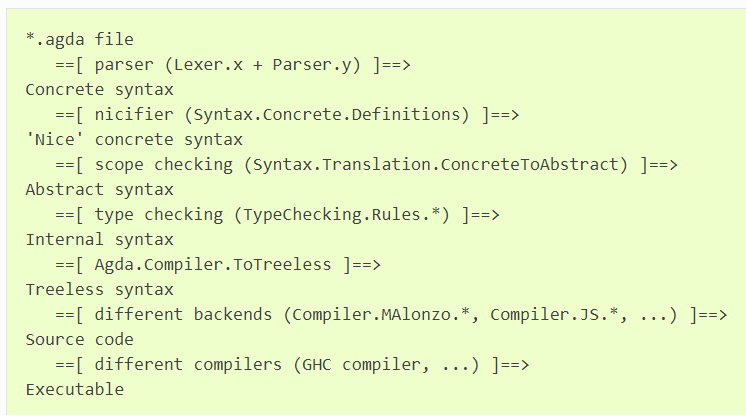
\includegraphics{agdaFileCompilation.png}
	\caption{Žingsniai kol Agda kodas yra paverčiamas kitos kalbos vykdomuoju failu \cite{AgdaWeb}}
	\centering
	\end{figure}
Pagal šį paveikslėlį matome, kad kompiliuojant Agda failą jis praeina pro tokias stadijas: 
\begin{itemize}
	\item Konkreti sintaksė - tai auškto lygio „cukruota“ (\textit{angl.} sugared) sintaksė, ji visiškai atitinka programuotojo įvestą kodą
	\item Abstrakti sintaksė - tai kodo versija prieš tipų patikrinimus, į ją įeina apimties analizė, operatorių pirmenybės išsiaiškinimas. Šioje reprezentacijoje yra atliekami tipų patikrinimai
	\item Vidinė sintaksė - tai paskutinis sintaksės transformavimo etapas prieš atiduodant ją posistemėms. Šiame etape termai yra tinkamai apibrėžti ir tinkamai tipizuoti. Kuriant vidinę sintaksę yra atliekami termų saugumo patikrinimai:
	\begin{itemize}
		\item Funkcijų baigtumo - patikrinama ar rekursiškai aprašytos funkcijos yra baigtinės.
		\item Duomenų tipų pozityvumo - užtikrinama, kad duomenų tipo indukcinio konstruktoriaus parametro argumentai nėra to paties tipo, kaip aprašomas duomenų tipas.
		\item Funkcijų apimties - patikrinama ar šablonų patikrinimas apima visus galimus variantus.
	\end{itemize}
	Vidinės sintaksės atvaizdavimui yra naudojamas Haskell duomenų tipas Term.
	\begin{figure}[H]
		\centering
		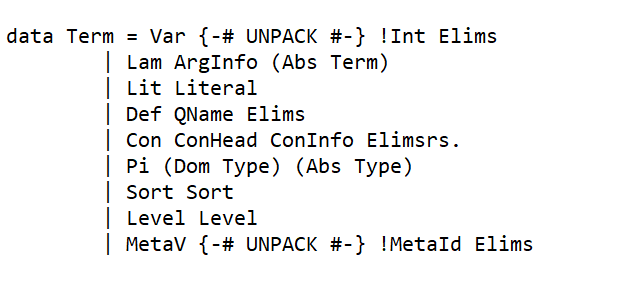
\includegraphics{HaskellTerm.png}
		\caption{Haskell duomenų tipas, kuris yra naudojamas vidinės sintaksės atvaizdavimui}
		\centering
		\end{figure}
		\item Bemedė sintaksė (\textit{angl.} Treeless syntax) - tai sintaksė, kuri skirta kompiliatoriaus posistemei (\textit{angl.} compiler backend) naudoti. Tai yra šiek tiek žemesnio lygio stuktūra negu vidinė sintaksė ir joje nėra atliekami tipų patikrinimai. Šioje sintakėse naudojama atvėjo išraiškos (\textit{angl.} case expressions) vietoje atvėjo medžių (\textit{angl.} case trees), kurie naudojami vidinėje sitaksėje. Šios išraiškos yra Agda funkcijos reprezentacija vidinėje bei bemedėje sintaksėje, iš esmės jos yra panašios, pagrindinis skirtumas yra tas, kad atvėjo išraiškos yra A-normalios formos (\textit{angl.} A-normal-form), tai reiškia, kad kiekvienam patikrinimui yra naudojamas tik vienas kintamasis, kai tuo tarpu atvėjo medžiuose gali būti naudojama ne vienas kintamasis. Žemiau galime matyti bemedę sintaksę išreikštą Haskell duomenų tipu „TTerm“:
		\begin{figure}[H]
			\centering
			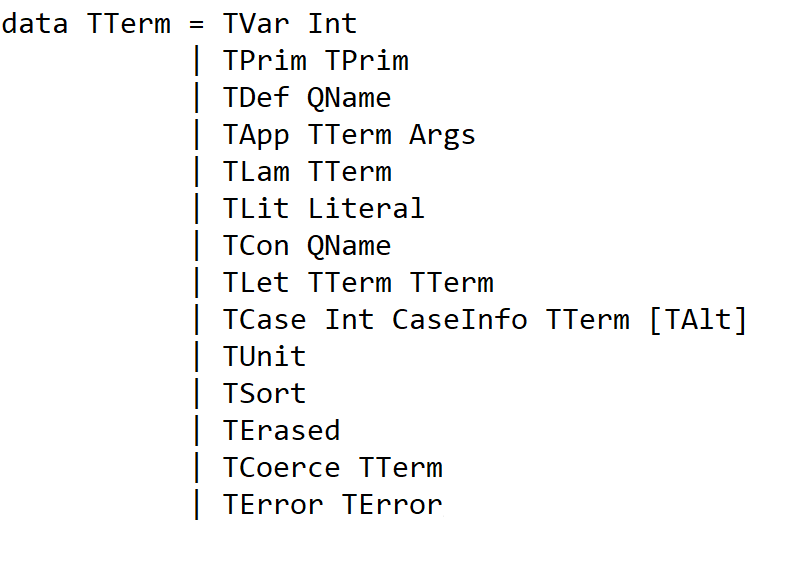
\includegraphics[scale=0.75]{TreelessTerm.png}
			\caption{Haskell duomenų tipas kuriuo išreikšta bemedė sintaksė}
			\label{img:tterm}
			\centering
			\end{figure}
\end{itemize}
Tarkime turime paprastą sudėties funkcija Agda kalboje:
\begin{lstlisting}
_+_ : Nat -> Nat -> Nat
zero + m = m
suc n + m = suc (n + m)
\end{lstlisting}
Pavertus į bemedę struktūrą ta pati funkcija atrodo taip:
\begin{lstlisting}
lambda a b ->
	case a of
		demo.Nat.zero -> b
		demo.Nat.suc c -> demo.Nat.suc (demo._+_ c b)
\end{lstlisting}
Čia matome, kad šioje stuktūroje turime atvėjo išraiškas po vieną kintamąjį, šablonų derinimas vyksta nurodant pilną konstruktoriaus vardą (šiuo atveju „demo“ yra modulio pavadinimas)
\subsection{Agda Duomenų tipų konvertavimas į Go}
Go programavimo kalba neturi nei indukcinių nei bendrinių algebrinių tipų, todėl reikia surasti reprezentaciją Go kalboje, kuri yra panašiausia į Agda indukcinius tipus.\par Vienas iš būdų, kaip galima aprašyti Bendrinius algebrinius tipus (arba indukcinius tipus) yra sąsajos (ang. interface) ir struktūros (ang. struct) pagalba. Tarkime turime sąrašo duomenų tipą Agda kalboje:
\begin{lstlisting}
data Vec (A : Set) : Nat -> Set where
	empty : Vec A zero
	append : {n : Nat} -> A -> Vec A n -> Vec A (suc n)
\end{lstlisting}
Iš esmės panašią struktūrą Go kalboje galima sukurti duomenų tipą pavertus į sąsają, o konstruktorius į struktūras:
\begin{lstlisting}[language=GoCust]
type Vec interface{}
type empty struct{}
type append struct {
	value interface{}
	tail Vec
}
\end{lstlisting}
Jeigu norėtume sukurti sąrašą iš 2 elementų Go kalboje, galėtume parašyti tokią eilutę: 
\begin{lstlisting}[language=GoCust]
append{1, append{4, empty{}}}
	\end{lstlisting}
Kadangi šioje struktūroje elementus saugome kaip „interface{}“ tipo elementus, gavę rezultatą bei norėdami naudoti funkcijas dirbančias su konkrečiu tipu, juos reikia paversti atgal į tipą, kuris buvo įdėtas į duomenų struktūrą.
\subsection{Agda funkcijų konvertavimas į Go}
\subsubsection{Vidinė Go sintaksės reprezentacija}
Norint transformuoti Agda kodą į kitos kalbos kodą paprastai naudojama tam tikra vidinė kodo reprezentaciją į kurią pirmiausia yra paverčiamas Agda kodas. Galime apribrėžti Haskell duomenų tipą, kuris reprezentuos Go kalbos poaibį, į kurį transformuojame Agda funkcijas:
\begin{figure}[H]
	\centering
	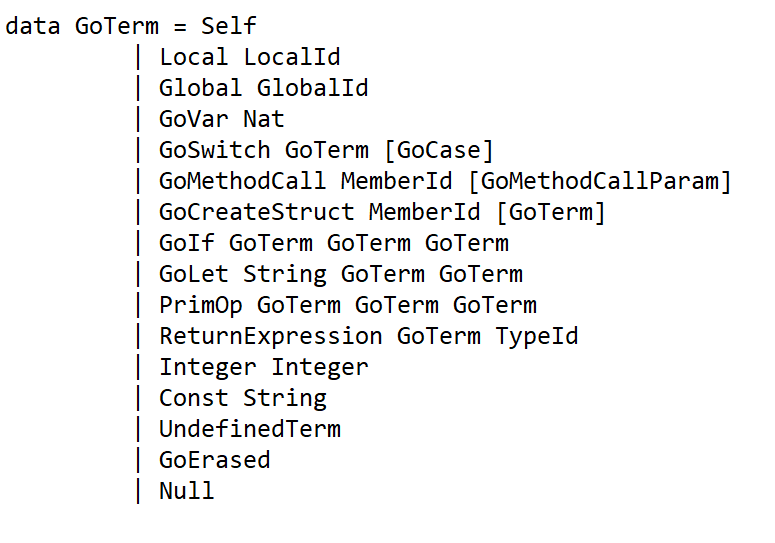
\includegraphics[scale=0.75]{GoTerm.png}
	\caption{Haskell duomenų tipas kuriuo išreikšta Go kalbos poaibio vidinė sintaksė}
	\label{img:goterm}
	\centering
	\end{figure}
Šis duomenų tipas veikia kaip tarpinė reprezentacija transformuojant Agda kodą į Go. Transformuojant Agda funkcijų kodą, jis pirmiausia yra paverčiamas į šią tarpinę reprezentaciją, iš kurios vėliau yra generuojamas Go kodas.
\par Anksčiau pademonstruotas Haskell duomenų tipas apibrėžiantis bemedę sintaksę (\ref{img:tterm} pav.) bei šis duomenų tipas (\ref{img:goterm} pav.) apibrėžia galimus funkcijos kūno elementus (be funkcijos aprašymo), taigi galime susieti šiuos du duomenų tipus nurodydami šiame darbe palaikomas transformavimo taisykles:
\begin{center}
	\begin{table}[h]
		\caption{Agda transformavimus vaizduojanti lentelė}
	\begin{tabular}{ |l|l| } 
	\hline
	\textbf{Bemedės struktūros Term reikšmė} & \textbf{Go Term reikšmė}  \\
	\hline
	TVar Int & GoVar Nat \\ 
	\hline
	TDef QName & GoMethodCall MemberId [] \\ 
	\hline
	TCase Int CaseInfo TTerm [TAlt] & GoSwitch GoVar [GoCase] \\ 
	\hline
	TApp TTerm(TDef) [TTerm] & GoMethodCall MemberId [GoMethodCallParam] \\ 
	\hline
	TApp TTerm(TCon) [TTerm] & GoCreateStruct MemberId [GoTerm] \\ 
	\hline
	TApp TTerm(TVar) [TTerm] & GoMethodCall GoVar [GoMethodCallParam] \\ 
	\hline
	TApp TTerm(TPrif PIf) [TTerm] & GoIf GoTerm GoTerm GoTerm \\ 
	\hline
	TApp TTerm(TPrim) [TTerm] & PrimOp GoTerm GoTerm GoTerm \\ 
	\hline
	TLet TTerm TTerm & GoLet GoTerm GoTerm \\ 
	\hline
	TLit Literal & GoLit GoLiteral \\ 
	\hline
	TCon QName & GoCreateStruct MemberId [] \\ 
	\hline
	TPrim TPrim & PrimOp GoTerm GoTerm GoTerm \\ 
	\hline
	\end{tabular}
\end{table}
	\end{center}
	Šioje lentelėje pažymėti atliekami transformavimai. Jeigu reikšmė įrašyta skliausteliuose, reiškia, kad tikrinama tipo konkreti reikšmė esanti skliausteliuose. Atlikus transformavimą iš bemedės struktūros į mūsų aprašytą Go termą vėliau yra generuojamas Go kodas
	\begin{itemize}
		\item GoVar a - kintamasis, kurio reikšmė yra 'a' simbolis, kurio reikšmė yra padidinta parametro „a“ reikšmės dydžiu. Pavyzdžiui jeigu a reikšmė yra 2, tada kintamojo vardas bus 'c'
		\item GoMethodCall merberId goTerms - Go metodo kvietimas, kur memberId yra metodo vardas, o goTerms yra šio metodo argumentai, kurie savyje laiko GoTerm bei, jeigu reikia, argumento tipą.
		\item GoSwtich goVar cases - tai yra Go „switch-case“ konstruktas, kur goVar nurodo kintamąjį, kurio reikšmė yra tikrinama, o cases apibrėžia galimus variantus
		\item GoCreateStruct memberId goTerms - Go struktūros kūrimas, kur memberId yra structūros vardas, o goTerms yra šios structūros elementų reikšmės
		\item GoIf term1 term2 term3 - Go sąlyginis sakinys, kur term1 yra primityvi if sakinio operacija, kuri gražina loginę reikšmę, pagal kurią yra vykdoma arba term2, arba term3 operacijos.
		\item PrimOp goTerm1 goTerm2 goTerm3 - Go primityvi operacija, kur goTerm1 apibrėžia primityvios operacijos tipą, o goTerm2 ir goTerm3 yra šios operacijos argumentai
		\item GoLet goTerm1 goTerm2 - tai naujo kintamojo sukūrimas, goTerm1 apibrėžia to kintamojo reikšmę, o goTerm2 yra tolesnę funkcijos operacija
		\item GoLit GoLiteral - tai primityvi reikšmė (šiuo metu palaikoma tik sveikojo skaičiaus reikšmė)
	\end{itemize}
\subsubsection{Paprastos funkcijos konvertavimas}
Tarkime naudojame tą patį sąrašą į kurį jau įdėti keli natūralieji skaičiai, norėdami sudėti tuos natūraliuosius skaičius, Agda kalboje tokios funkcijos atrodytų taip:
\begin{lstlisting}
add : Nat -> Nat -> Nat
add zero m = m
add (suc n) m = suc (n + m)

sum : List Nat -> Nat
sum empty = zero
sum (append value tail) = add value (sum tail)
\end{lstlisting}
Go programavimo kalboje galėtume sukurti tokius metodus:
\begin{lstlisting}[language=GoCust]
func add(a interface{}) func(interface{}) Nat {
	return func(b interface{}) Nat {
		switch type_a := a.(type) {
			case Nat_zero:
				return b
			case Nat_suc:
				c := type_a._1
				_ = c
				return Nat_suc{add(c)(b)}
			default:
				_ = type_a
				panic("Unreachable")
		}
	}
}
func sum(a List) Nat {
  switch type_a := a.(type) {
  case List_empty:
    return Nat_zero{}
	case List_append : 
		b := type_a.a;
		 _ = b;
		c := type_a.b;
		 _ = c;
    return add(sum(c))(b)
  default:
    panic("error")
  }
}
	\end{lstlisting}
	Kur natūralusis skaičius apibrėžtas taip:
	\begin{lstlisting}[language=GoCust]
type Nat interface{}
type Nat_zero struct{}
type Nat_suc struct {
	value Nat
}
\end{lstlisting}

Pirmojoje Go funkcijoje matome, kad funkcijos yra suskaidytos į mažesnes funkcijas po vieną argumentą, kad atitiktų funkcinio programavimo principus ir esant poreikiui į kitą metodą būtų galima paduoti funkcija add(5), kuri prie duoto natūraliojo skaičiaus prideda 5. Tačiau toks užrašymas prideda sudėtingumo funkcijoms, kadangi Go kalboje privaloma tiksliai nurodyti funkcijos grąžinimo tipą, taigi kuo daugiau parametrų priima funkcija, tuo labiau išsiplečia jos grąžinamas tipas.
\subsubsection{Standartiniai tipai}
Agda kalboje pragmų pagalba yra įmanoma nurodyti tam tikrų tipų atitikmenis Haskell kalboje, tuo galima pasinaudoti ir konvertuodami kodą į Go. Prie natūraliojo skaičiaus duomenų tipo pridėjus eilutę 
\begin{lstlisting}
{-# BUILTIN NATURAL Nat #-}
\end{lstlisting}
Transliavimo metu galime nurodyti į kokį konkrečiai tipą reikia konvertuoti labiausiai naudojamus tipus, tokius kaip sveikieji skaičiai, sąrašai ar loginis tipas. Šios pragmos yra skirtos transliavimui į Haskell kalbą, tačiau dalį jų galime panaudoti ir transliavime į Go. \par Konvertuodami natūraliuosius skaičius į Go programavimo kalbą turime kelis variantus:
\begin{itemize}
	\item Primityvus tipas „int“
	\item Didelių skaičių biblioteka „math“, kuri turi „bigInt“ tipą
	\item C kalbos bibliotekos „gmp“ sveikojo skaičiaus todo kuris yra sukurtas kaip  „bigInt“ bibliotekos alternatyva.
\end{itemize}
Primityvus tipas yra greitesnis už šias bibliotekas, tačiau yra stipriai ribojamas maksimalaus skaičiaus dydžio, todėl norint kad duomenų tipas atitiktų Agda duomenų tipą, šiame darbe renkamasi tarp math ir gmp bibliotekų. Galime palyginti šių bibliotekų našumą skaičiuodami faktorialo funkciją dideliems skaičiams:
\begin{center}
	\centering
	\begin{table}[H]
		\caption{„math“ ir „gmp“ bibliotekų faktorialo skaičiavimo efektyvumo palyginimas}
		\centering
	\begin{tabular}{ ccc } 
	\toprule
	& \textbf{math} & \textbf{gmp}  \\
	\midrule
	n = 100 & 0.02ms & 0.31ms    \\
	\midrule
	n = 1000 & 0.39ms & 3.41ms  \\
	\midrule
	n = 10000 & 38.85ms & 54.57ms  \\
	\midrule
	n = 100000 & 18.58s & 10.86s  \\
	\bottomrule
	\end{tabular}
	\centering
\end{table}
	\end{center}
	Kaip matome šioje lentelėje, „math“ biblioteka veikia efektyviau su mažesniais skaičiais ir tik su pačiais didžiausiais skaičiais veikia lėčiau negu „gmp“ biblioteka. Tačiau santykinis skirtumas yra didesnis skaičiuojant mažesnes reikšmes, todėl šiame darbe buvo pasirinkta naudoti „math“ bibliotekos „bigInt“ tipą Agda natūraliesiems skaičiams atvaizduoti.
\par Panaudojus pragmą, su kuria nurodome į kokį tipą transliuojame natūralųjį skaičių, taip pat turime nurodyti metodų atitikmenis, kurie yra skirti dirbti su šiuo primityviu tipu, tai tokios operacijos kaip sudėtis, atimtis, daugyba, dalyba bei lygybė. Šiam tikslui pasiekti buvo sukurtas pagalbinis paketas, kurio metodai yra kviečiami norint atlikti aukščiau paminėtas operacijas. Pavyzdžiui, prie tai aprašytame „Nat“ duomenų tipo aprašyme nurodę, kad tai yra standartinis natūralusis skaičius, gauname tokį prieš tai aprašytą sudėties metodą:
\begin{lstlisting}[language=GoCust]
func add(a interface{}) func(interface{}) *big.Int {
	return func(b interface{}) *big.Int {
 		if ( helper.Equals((big.NewInt(0)),(a)) ) {
 			return b.(*big.Int) 
		} else {
 			c := helper.Minus((a),(big.NewInt(1))) 
 			return helper.Add((big.NewInt(1)),(add(c) (b))).(*big.Int) 
		}
 	}
}
\end{lstlisting}
Šiame metode naudojamas mūsų nurodytas Go kalboje egzituojantis tipas, kuris yra tinkamas saugoti natūraliesiems skaičiams.
\subsubsection{Bendrinių tipų konvertavimas}
Bendriniai tipai šioje realizacijoje būtini transliuojant funkcijas, kurios vienas iš parametrų yra funkcijos tipo. Pavyzdžiui, jeigu turime funkciją „Map“, kuri pritaiko tam tikrą funkciją kiekvienam sąrašo elementui, vienas būdas ją transformuoti į Go būtų paverčiant visų argumentų tipus į „interface{}“ tipą:
\begin{lstlisting}[language=GoCust]
func Map(a func(interface{}) interface{}) func(List) List {
	return func(b List) List {
		. . . .
	}
}
\end{lstlisting}
Tačiau šiuo atveju „Map“ funkciją galėtume kviesti perduodami tik tuos metodus, kurie priima ir grąžina „interface{}“ tipo elementus. Todėl, jeigu turėtume sąrašą sveikųjų skaičių ir norime prie jų pridėti 5, negalime pasinaudoti jau aprašyta funkcija „add“, kadangi, jeigu į „Map“ perduotume pirmą parametrą „add(NewInt(5))“, gautume kompiliavimo klaidą, nes nesutaptų priimamos ir perduodamos funkcijų aprašai. Šiai problemai išspręsti galime pasinaudoti bendriniais tipais iš prieš tai minėto pasiūlymo. Tuo atveju „Map“ funkciją galima būtų aprašyti taip:
\begin{lstlisting}[language=GoCust]
	func Map[T1, T0 any](a func(T1) T0) func(List) List {
		return func(b List) List {
			. . . .
		}
	}
	\end{lstlisting}
Taip aprašius funkciją, kompiliuodami Go kodą, sugeneruosime skirtingas „Map“ variacijas kiekvienam kvietimui kuris perduoda funkciją su skirtingu aprašu.
\subsubsection{Raktinio žodžio „return“ pridėjimas}
Transliavimo metu yra sudėtinga nustatyti, kurioje vietoje naudoti „return“ raktinį žodį, kadangi tuo metu dar nėra aišku, kokia tiksliai operacija bus naudojama ir ar tai yra paskutinė operacija šakoje. Šiai situacijai išspręsti, po metodo transliavimo yra kviečiama funkcija, kuri pereina per visą medį, tikrindama ar operacija toje šakoje yra paskutinė. Šiam tikslui pasiekti buvo apsibrėžtas sąrašas, kuris nurodo operacijas, kurios grąžina konkrečią reikšmę, tai tokios operacijos kaip metodo kvietimas, struktūros sukūrimas ar tiesiog kintamojo grąžinimas. Jeigu operacija yra paskutinė, tada tos operacijos duomenų tipas yra apvelkamas nauju tipu \mbox{ „ReturnExpression“}, kuris kodo generatoriui nurodo, kad ši operacija pradžioje turi turėti „return“ raktinį žodį. \par Taip pat, kaip matoma Go tarpinės reprezentacijos Haskell duomenų tipe (\ref{img:goterm} pav.), „ReturnExpression“ tipas taip pat saugo grąžinamo tipo informaciją. Tai yra reikalinga norint užtikrinti, kad grąžinamas toks tipas, kurį nurodo metodo aprašymas.
\subsection{Įrodymai}
Transliuoti įrodymų iš Agda programavimo kalbos į Go nėra reikalinga bei prasminga, tai nėra daroma nei MAlonzo, nei JavaScript transliatoriuose. Verčiant šių funkcijų kodą iš Agda abstrakčios sintaksės į bemedę yra gaunamas rezultatas „TErased“, kuris nusako, kad tokia funkcija gali būti pašalinta.
\subsection{Visų kintamųjų bei importuotų bibliotekų panaudojimas}
Kadangi Go neleidžia kompiliuoti kodo, kuriame yra nenaudojamų kintamųjų ar importuotų bibliotekų, transliuodami Agda kodą privalome užtikrinti, kad tokių situacijų neatsitiktų. Kaip jau buvo galima matyti Go kodo pavyzdžiuose, transliuodami Agda koda yra parašome priskyrimą, pavyzdžiui, „\_ = c“. Ši eilutė reiškia, kad kintamasis „c“ yra priskiriamas tuščiam identifikatoriui.\par Transliuodami Agda kodą taip pat galime susidurti su situacija, kai nurodomos bibliotekos, kurios tame pakete nėra naudojamos. Norint išvengti tokių klaidų, transliavimo metu kiekviename pakete pridedame papildomą tipo kintamąjį „type GoImportable int“. Šis kintamasis yra panaudojamas kiekviename pakete, kuris importuoja kitą paketą. Tarkime, turime „package a“ ir „package b“, kur paketas a importuoja paketą „b“, tada paketo „a“ kode pridėsime eilutę „type \_ a.GoImportable“. Ši eilutė užtikrina, kad Go kompiliatorius neišmes klaidos dėl nenaudojamos importuotos bibliotekos.
\subsection{Simbolių užkodavimas verčiant į Go}
Kaip jau buvo minėta ankstesniame skyriuje, Agda leidžia praktiškai bet kokius vardus funkcijoms, bei duomenų tipams, kai tuo tarpu Go kalboje jie yra žymiai labiau ribojami. MAlonzo kompiliatoriuje į Haskell tai apeinama duomenų struktūroms, konstruktoriams, bei funkcijoms įvardinti naudojant naujai sukurtus vardus, pavyzdžiui:
\begin{lstlisting}
name2 = "demo.Nat"
d2 = ()
data T2 = C4 | C6 T2
\end{lstlisting}
kur d2 yra funkcijos vardas, T2 yra duomenų tipo vardas, o name2 yra eilutės tipo kintamasis, kuris saugo funkcijos vardą Agda kode. Toks metodas yra tinkamas, kai yra generuojamas vykdomasis failas, bet norint sugeneruoti kodą, kuris yra kviečiamas iš Go kodo toks sprendimas yra netinkamas. \par Paprasčiausias sprendimas šiam klausimui būtų apriboti simbolius, kuriuos galima naudoti rašant Agda kodą. Tačiau tuo atveju norėdami transliuoti Agda standartinės bibliotekos kodą susiduriame su problemomis, kadangi nėra galimybių perrašyti visą standartinės bibliotekos kodą pakeičiant visus Go kalboje nepriimamus simbolius. Šiai problemai apeiti galime sukurti užkodavimą, kuris transliavimo metu patikrina ar kiekvienas transliuojamas simbolis yra apatinis brūkšnys arba „unicode“ raidės simbolis. Jeigu ši sąlygą yra nepatenkinama, tada simbolį verčiame į jo dešimtainio skaičiaus reprezentaciją, prie jos pridedami raidę „u“, pavyzdžiui, versdami dolerio ženklą „\$“, gauname kodą „u36“.
\section{Našumo testai}
Šiame skyriuje aprašomi 3 skirtingų funkcijų veikimo greičio bei atminties naudojimo palyginimai. Lyginimas atliekamas tarp Agda kodo sugeneruoto į Go bei kodo sugeneruoto į Haskell naudojantis Malonnzo kompiliatoriumi. Visi palyginimai buvo leidžiami kompiuteryje su  „AMD Ryzen 7 3750H“ procesoriumi, bei 16GB atminties. Go kalboje matavimai atlikti naudojantis baziniu „testing“ paketu, o Haskell kalboje „criterion“ bei „weigth“ bibliotekomis. 
\par Pirmasis testas atliktas su faktorialo funkcija (žr. \ref{sec:priedas2} priedas): 
\begin{center}
	\centering
	\begin{table}[H]
		\caption{Go ir Haskell faktorialo skaičiavimo efektyvumo palyginimas}
		\centering
	\begin{tabular}{ cccc } 
	& & \textbf{Go} & \textbf{Haskell}  \\
	\midrule
	n = 100 & laikas & 0.02ms & 0.0044ms    \\
	& atmintis & 11.6KB & 9.25KB \\
	\midrule
	n = 1000 & laikas & 0.39ms & 0.12ms  \\
	& atmintis & 0.59MB & 0.63MB \\
	\midrule
	n = 10000 & laikas & 38.85ms & 11.78ms  \\
	& atmintis & 74.4MB & 84.11MB \\
	\midrule
	n = 100000 & laikas & 18.58s & 1.35s  \\
	& atmintis & 9.38GB & 11.28GB \\
	\end{tabular}
	\centering
\end{table}
\end{center}
	Kaip matoma šioje lentelėje, Haskell veikia greičiau su visais n, tačiau Go kodas naudoja mažiau atminties pasiekus n = 100000. 
	\par Antrasis testas skaičiuoja pirminių skaičių kiekį iki duoto natūralausiaus skaičiaus n (žr. \ref{sec:priedas3} priedas). Kaip matoma lentelėje žemiau, Ši funkcija paversta į Go, palyginus su Haskell, veikia labai lėtai, su n reikšme 1000, nėra gaunamas rezultatas kadangi pritrūkstama atminties.
	\begin{center}
		\centering
		\begin{table}[h]
			\caption{Go ir Haskell pirminių skaičių kieko radimo funckija}
			\centering
		\begin{tabular}{ cccc } 
		& & \textbf{Go} & \textbf{Haskell}  \\
		\midrule
		n = 100 & laikas & 27.07ms & 0.15ms    \\
		& atmintis & 8.75MB & 0.17MB \\
		\midrule
		n = 500 & laikas & 44.7s & 3.24ms  \\
		& atmintis & 13.7GB & 4MB \\
		\midrule
		n = 1000 & laikas & - & 13.07ms  \\
		& atmintis & - & 16.1MB \\
		\end{tabular}
		\centering
	\end{table}
		\end{center}
		Atlikus analizę buvo pastebėta, kad didžioji dalis laiko yra sunaudojama rekursiniuose kvietimuose todėl, kad „let“ išraiškoje yra priskiriamas metodo iškvietimas. Tai nesukelia problemų Haskell kalboje, kadangi  yra taikomas tingus inicializavimus, kurio dėka reikšmė nėra skaičiuojama, kol ji nėra naudojama. Šiaip problemai išspręsti siųlomas pakeitimas, nepriskirti medoto kvietimo kintamąjam, tačiau jį pridėti toje vietoje, kur yra naudojamas tas kintamasis. Atlikus šį pakeitimą pirminių skaičiaus kieko skaičiavimo funkcijoje gaunami žymiai geresni rezultatai:
		\begin{center}
			\centering
			\begin{table}[h]
				\caption{Go ir Haskell pirminių skaičių kieko radimo funckija}
				\centering
			\begin{tabular}{ cccc } 
			& & \textbf{Go} & \textbf{Haskell}  \\
			\midrule
			n = 100 & laikas & 1.86ms & 0.15ms    \\
			& atmintis & 0.65MB & 0.17MB \\
			\midrule
			n = 500 & laikas & 44.24ms & 3.24ms  \\
			& atmintis & 15.33MB & 4MB \\
			\midrule
			n = 1000 & laikas & 178ms & 13.07ms  \\
			& atmintis & 60.7MB & 16.1MB \\
			\midrule
			n = 10000 & laikas & 19.9s & 1.27s  \\
			& atmintis & 6GB & 1.6GB \\
			\end{tabular}
			\centering
		\end{table}
			\end{center}

			\par Trečiasis testas atliktas leidžiant funkciją, kuri burburo rikiavimo metodu surikiuoja duotą sąrašą (žr. \ref{sec:priedas4} priedas). Visų šio sąrašo elementų dydis yra iki 10.
			\begin{center}
				\centering
				\begin{table}[h]
					\caption{Go ir Haskell bubble sort funkcija}
					\centering
				\begin{tabular}{ cccc } 
				& & \textbf{Go} & \textbf{Haskell}  \\
				\midrule
				n = 100 & laikas & 19.24ms & 0.81ms    \\
				 & atmintis & 57.78MB & pending  \\
				\midrule
				n = 1000 & laikas & 1.93s & 0.09s  \\
				 & atmintis & 6.16GB & pending \\
				\midrule
				\end{tabular}
				\centering
			\end{table}
				\end{center}
Galime matyti, kad rezultatai santykinai yra prastesni negu prieš tai leistų funkcijų. Buvo pastebėta, kad didelė dalis laiko, iki 30\%, yra išnaudojama atliekant šiukšlių surinkimą (\textit{angl.} garbage collection). Taip pat, veikimo greitis numatomai turėtų žymiai pagreitėti implementavus išorinę funkcijos sąsaja bei šį vektoriaus tipą pavertus į Go sąrašo tipą.
\section{Verifikavimas}

\sectionnonum{Ateities darbai}
\begin{enumerate}[noitemsep]
  \item Išorinė funkcijos sąsaja. Šiuo metu nėra galimybės tiesiogiai susieti Agda funkcijų bei duomenų tipų su konkrečiais Go kalbos elementais. Tam tikslui pasiekti yra reikalinga išorinė funkcijos sąsaja, su kuria pragmu pagalba būtų galima nurodyti kokia Go funkcija ar struktūra atitinka pasirinktas Agda funkcijas ar duomenų tipus.
  \item Bendriniai duomenų tipai. Šiuo metu transformuojami Agda duomenų tipai yra paverčiami į tokius duomenų tipas, kurių laukai yra tuščios sąsajos tipo, tai reiškia, kad metodai dirbantys su jais, savo aprašyme negali naudoti bendrinių tipų. Tai iš dalies galėtų būti sprendžiama išorinės funkcijos sąsajos pagalba tam tikrus tipus verčiant į jau egzistuojančias Go struktūras, tačiau norint naudotis visais Agda privalumais yra reikalingi bendriniai duomenų tipai  aprašyti Go kalboje.
  \item Įgyvendinti įrašo tipų transliavimą. 
  \item Įgyvendinti automatinį Go modulio sukūrimą ar paketų perkėlimą į Go bibliotekų aplanką. Importuojant skirtingus Go paketus, jie yra imami arba iš go bibliotekų aplanko, arba, jeigu yra nurodytas modulis, iš modulio aplanko. Dėl šios priežasties reikalingas funkcionalumas, kuris leidžia arba perkelti sukompiliuotas klases į Go bibliotekų aplanką, jeigu jos yra bendros visiems projektams, arba sukurti Go modulį, kad to nereikėtų kiekvieną kartą daryti rankinių būdu.
\end{enumerate}
\sectionnonum{Rezultatai}
\begin{enumerate}[noitemsep]
  \item Aprašytos Agda funkcijų transformavimo taisyklės
  \item Įgyvendintos aprašytos taisyklės
  \item Pateikti našumo palyginimai tarp Go ir Haskell sugeneruotų programų
  \item Nurodyti esamo transliatoriaus trūkumai
  \item Pateikti siūlomi ateities darbai
\end{enumerate}
\sectionnonum{Išvados}
\begin{enumerate}[noitemsep]
  \item Agda kodą galima transliuoti į Go kalbos kodą
  \item Su šiuo transliatoriaus įgyvendinimu sugeneruotas kodas veikia 15-20 kartų lečiau, negu kodas sugeneruotas į Haskell
\end{enumerate}

\printbibliography[heading=bibintoc] 

	\sectionnonum{1 priedas. Agda kodas paverstas į kitas kalbas}
	\label{sec:priedas1}
	Agda sąrašo tipas ir funkcijos, kurios sudeda sąrašo elementus ir grąžina natūralūjį skaičių paverstos į Haskell ir Javascript kalbas. \newline
	Haskell:
	\begin{lstlisting}
	name46 = "demo.List"
	d46 a0 = ()
	data T46 = C50 | C52 AgdaAny T46	
	name36 = "demo.add"
	d36 :: Integer -> Integer -> Integer
	d36 v0 v1
		= case coe v0 of
				0 -> coe v1
				_ -> let v2 = subInt (coe v0) (coe (1 :: Integer)) in
							coe addInt (coe (1 :: Integer)) (coe d24 (coe v2) (coe v1))
	name54 = "demo.sum"
	d54 :: T46 -> Integer
	d54 v0
		= case coe v0 of
				C50 -> coe (0 :: Integer)
				C52 v1 v2 -> coe d36 (coe v1) (coe d54 (coe v2))
				_ -> MAlonzo.RTE.mazUnreachableError
		\end{lstlisting}
	JavaScript:
	\begin{lstlisting}
	exports["List"] = {};
	exports["List"]["empty"] = a => a["empty"]();
	exports["List"]["append"] = a => b => c => c["append"](a,b);
	exports["add"] = a => b => (
		agdaRTS.uprimIntegerEqual(agdaRTS.primIntegerFromString("0"),a)? b: agdaRTS.uprimIntegerPlus(
			agdaRTS.primIntegerFromString("1"),
			exports["_+_"](
				agdaRTS.uprimIntegerMinus(a,agdaRTS.primIntegerFromString("1"))
			)(b)
		)
		);
	exports["sum"] = a => a({
			"append": (b,c) => exports["add"](b)(exports["sum"](c)),
			"empty": () => agdaRTS.primIntegerFromString("0")
		});
		\end{lstlisting}	

		\sectionnonum{2 priedas. Agda faktorialo funkcija paversta į kitas kalbas}
\label{sec:priedas2}
Agda faktorialo funkcija paverstą į Haskell ir Go. \newline
Agda:
\begin{lstlisting}
	_! : Nat -> Nat
	0 ! = 1
	(suc n) ! = (suc n) * (n !)
	\end{lstlisting}
Haskell:
\begin{lstlisting}
	name32 = "demo._!"
	d32 :: Integer -> Integer
	d32 v0
		= case coe v0 of
				0 -> coe (1 :: Integer)
				_ -> let v1 = subInt (coe v0) (coe (1 :: Integer)) in
						 coe mulInt (coe v0) (coe d32 (coe v1))
	\end{lstlisting}
Go:
	\begin{lstlisting}[language=GoCust]
		func F_u33(A interface{}) *big.Int {
			if helper.Equals((big.NewInt(0)), (A)) {
				return helper.Id(big.NewInt(1)).(*big.Int)
			} else {
				B := helper.Minus((A), (big.NewInt(1)))
				return helper.Id(helper.Multiply((A), (F_u33(B)))).(*big.Int)
			}
	\end{lstlisting}


	\sectionnonum{3 priedas. Agda pirminių skaičiaus kieko radimo funkcija paversta į kitas kalbas}
\label{sec:priedas3}
Agda pirminių skaičiaus kiekio radimo funkcija paverstą į Haskell ir Go. \newline
Agda:
\begin{lstlisting}
isPrime : Nat -> Bool
isPrime 0 = false
isPrime 1 = false
isPrime n with dividersCount n n
  where
  dividersCount : Nat -> Nat -> Nat
  dividersCount 0 _ = 0
  dividersCount _ 0 = 0
  dividersCount (suc n) m with mod-helper 0 n m n
  dividersCount (suc n) m | 0 = suc (dividersCount n m)
  dividersCount (suc n) m | _ = dividersCount n m
isPrime n | 2 = true
isPrime n | _ = false  

countPrimes : Nat -> Nat
countPrimes 0 = 0
countPrimes (suc n) with isPrime (suc n)
countPrimes (suc n) | false = countPrimes n
countPrimes (suc n) | true = suc (countPrimes n)
	\end{lstlisting}
Haskell:
\begin{lstlisting}
name290 = "demo.isPrime"
d290 :: Integer -> Bool
d290 v0
	= let v1
					= let v1 = coe du298 (coe v0) (coe v0) in
						case coe v1 of
							2 -> coe MAlonzo.Code.Agda.Builtin.Bool.C10
							_ | coe geqInt (coe v1) (coe (2 :: Integer)) ->
									coe MAlonzo.Code.Agda.Builtin.Bool.C8
							1 -> coe MAlonzo.Code.Agda.Builtin.Bool.C8
							_ -> coe MAlonzo.Code.Agda.Builtin.Bool.C8 in
		case coe v0 of
			0 -> coe MAlonzo.Code.Agda.Builtin.Bool.C8
			1 -> coe MAlonzo.Code.Agda.Builtin.Bool.C8
			_ -> coe v1
name298 = "demo._.dividersCount"
d298 :: Integer -> Integer -> Integer -> Integer
d298 v0 v1 v2 = du298 v1 v2
du298 :: Integer -> Integer -> Integer
du298 v0 v1
	= case coe v0 of
			0 -> coe (0 :: Integer)
			_ -> let v2 = subInt (coe v0) (coe (1 :: Integer)) in
						let v3
									= let v3 = remInt (coe v1) (coe v0) in
										let v4 = coe du298 (coe v2) (coe v1) in
										case coe v3 of
											0 -> coe addInt (coe (1 :: Integer)) (coe du298 (coe v2) (coe v1))
											_ -> coe v4 in
						case coe v1 of
							0 -> coe (0 :: Integer)
							_ -> coe v3
name324 = "demo.countPrimes"
d324 :: Integer -> Integer
d324 v0
	= case coe v0 of
			0 -> coe (0 :: Integer)
			_ -> let v1 = subInt (coe v0) (coe (1 :: Integer)) in
						let v2 = d290 (coe v0) in
						if coe v2
							then coe addInt (coe (1 :: Integer)) (coe d324 (coe v1))
							else coe d324 (coe v1)
	\end{lstlisting}
Go:
\begin{lstlisting}[language=GoCust]
func FisPrime(A interface{}) Agda_Builtin_Bool.Bool {
	B := F_NameIdu32296u321274468892439276514_dividersCount(A)(A)
	if helper.Equals((big.NewInt(2)), (B)) {
		return helper.Id(Agda_Builtin_Bool.Bool_true{}).(Agda_Builtin_Bool.Bool)
	} else {
		if helper.Equals((big.NewInt(1)), (B)) {
			return helper.Id(Agda_Builtin_Bool.Bool_false{}).(Agda_Builtin_Bool.Bool)
		} else {
			if helper.MoreOrEquals((B), (big.NewInt(2))) {
				return helper.Id(Agda_Builtin_Bool.Bool_false{}).(Agda_Builtin_Bool.Bool)
			} else {
				return helper.Id(Agda_Builtin_Bool.Bool_false{}).(Agda_Builtin_Bool.Bool)
			}
		}
	}

	if helper.Equals((big.NewInt(0)), (A)) {
		return helper.Id(Agda_Builtin_Bool.Bool_false{}).(Agda_Builtin_Bool.Bool)
	} else {
		if helper.Equals((big.NewInt(1)), (A)) {
			return helper.Id(Agda_Builtin_Bool.Bool_false{}).(Agda_Builtin_Bool.Bool)
		} else {
			return helper.Id(B).(Agda_Builtin_Bool.Bool)
		}

	}
}

func F_NameIdu32296u321274468892439276514_dividersCount(A interface{}) func(interface{}) *big.Int {
	return func(B interface{}) *big.Int {
		if helper.Equals((big.NewInt(0)), (A)) {
			return helper.Id(big.NewInt(0)).(*big.Int)
		} else {
			C := helper.Minus((A), (big.NewInt(1)))
			D := helper.Mod((B), (A))
			E := F_NameIdu32296u321274468892439276514_dividersCount(C)(B)
			if helper.Equals((big.NewInt(0)), (D)) {
				return helper.Id(helper.Add((big.NewInt(1)), (F_NameIdu32296u321274468892439276514_dividersCount(C)(B)))).(*big.Int)
			} else {
				return helper.Id(E).(*big.Int)
			}
			if helper.Equals((big.NewInt(0)), (B)) {
				return helper.Id(big.NewInt(0)).(*big.Int)
			} else {
				return helper.Id(D).(*big.Int)
			}

		}
	}
}

func FcountPrimes(A interface{}) *big.Int {
	if helper.Equals((big.NewInt(0)), (A)) {
		return helper.Id(big.NewInt(0)).(*big.Int)
	} else {
		B := helper.Minus((A), (big.NewInt(1)))
		C := FisPrime(A)
		switch type_C := C.(type) {
		case Agda_Builtin_Bool.Bool_false:
		return helper.Id(FcountPrimes(B)).(*big.Int)
		case Agda_Builtin_Bool.Bool_true:
		return helper.Id(helper.Add((big.NewInt(1)), (FcountPrimes(B)))).(*big.Int)
		default:
			_ = type_C
			panic("Unreachable")
		}
	}
}
\end{lstlisting}


	\sectionnonum{4 priedas. Agda rikiavimo funkcija paversta į kitas kalbas}
\label{sec:priedas4}
Agda sąrašo rikiavimo funkcija paverstą į Haskell ir Go. \newline
Agda:
\begin{lstlisting}
	{-# TERMINATING #-}
	bubblesortiter : ∀ {n} -> Vec Nat n -> Vec Nat n
	bubblesortiter (appendV x (appendV y xs)) with  x > y
	bubblesortiter (appendV x (appendV y xs)) | true  = appendV y (bubblesortiter (appendV x xs))
	bubblesortiter (appendV x (appendV y xs)) | false  = appendV x (bubblesortiter (appendV y xs))
	bubblesortiter x = x
	
	
	{-# TERMINATING #-}
	bubblesort' : ∀ {n} -> Vec Nat n -> Nat -> Vec Nat n
	bubblesort' {n} xs i  with n eq i
	bubblesort' {n} xs i | true = xs
	bubblesort' {n} xs i | false = bubblesort' (bubblesortiter xs) (suc i)
	 
	bubblesort : ∀ {n} -> Vec Nat n -> Vec Nat n
	bubblesort xs = bubblesort' xs 0
	\end{lstlisting}
Haskell:
\begin{lstlisting}
name338 = "demo.bubblesortiter"
d338 :: Integer -> T152 -> T152
d338 v0 v1
	= case coe v1 of
			C160 v3 v4
				-> case coe v0 of
							_ | coe geqInt (coe v0) (coe (1 :: Integer)) ->
									case coe v4 of
										C160 v6 v7
											-> case coe v0 of
													_ | coe geqInt (coe v0) (coe (2 :: Integer)) ->
															let v8 = d12 (coe v3) (coe v6) in
															if coe v8
																then coe
																				C160 v6
																				(d338
																					(coe subInt (coe v0) (coe (1 :: Integer)))
																					(coe C160 v3 v7))
																else coe
																				C160 v3
																				(d338
																					(coe subInt (coe v0) (coe (1 :: Integer)))
																					(coe C160 v6 v7))
													_ -> coe v1
										_ -> coe v1
							_ -> coe v1
			_ -> coe v1
name366 = "demo.bubblesort'"
d366 :: Integer -> T152 -> Integer -> T152
d366 v0 v1 v2
	= let v3 = d22 (coe v0) (coe v2) in
		if coe v3
			then coe v1
			else coe
							d366 (coe v0) (coe d338 (coe v0) (coe v1))
							(coe addInt (coe (1 :: Integer)) (coe v2))
name392 = "demo.bubblesort"
d392 :: Integer -> T152 -> T152
d392 v0 v1 = coe d366 (coe v0) (coe v1) (coe (0 :: Integer))
\end{lstlisting}
Go:
\begin{lstlisting}[language=GoCust]
func Fbubblesortiter(A interface{}) func(Vec) Vec {
	return func(B Vec) Vec {
		C := B
		switch type_B := B.(type) {
		case Vec_appendV:
			D := type_B.A
			_ = D
			E := type_B.B
			_ = E
			if helper.MoreOrEquals((A), (big.NewInt(1))) {
				F := B
				switch type_E := E.(type) {
				case Vec_appendV:
					G := type_E.A
					_ = G
					H := type_E.B
					_ = H
					if helper.MoreOrEquals((A), (big.NewInt(2))) {
						I := F_u62_(D)(G)
						switch type_I := I.(type) {
						case Agda_Builtin_Bool.Bool_false:
				return helper.Id(Vec_appendV{D, Fbubblesortiter(helper.Minus((A), (big.NewInt(1))))(Vec_appendV{G, H})}).(Vec)
						case Agda_Builtin_Bool.Bool_true:
				return helper.Id(Vec_appendV{G, Fbubblesortiter(helper.Minus((A), (big.NewInt(1))))(Vec_appendV{D, H})}).(Vec)
						default:
							_ = type_I
							panic("Unreachable")
						}
					} else {
						return helper.Id(B).(Vec)
					}
		case Vec_emptyV:
			return helper.Id(F).(Vec)
				default:
					_ = type_E
					panic("Unreachable")
				}
			} else {
				return helper.Id(B).(Vec)
			}
	case Vec_emptyV:
		return helper.Id(C).(Vec)
		default:
			_ = type_B
			panic("Unreachable")
		}
	}
}
func Fbubblesortu39(A interface{}) func(Vec) func(interface{}) Vec {
	return func(B Vec) func(interface{}) Vec {
		return func(C interface{}) Vec {
			D := F_eq_(A)(C)
			switch type_D := D.(type) {
			case Agda_Builtin_Bool.Bool_false:
		return helper.Id(Fbubblesortu39(A)(Fbubblesortiter(A)(B))(helper.Add((big.NewInt(1)), (C)))).(Vec)
			case Agda_Builtin_Bool.Bool_true:
		return helper.Id(B).(Vec)
			default:
				_ = type_D
				panic("Unreachable")
			}
	}
	}
}
func Fbubblesort(A interface{}) func(Vec) Vec {
	return func(B Vec) Vec {
		return helper.Id(Fbubblesortu39(A)(B)(big.NewInt(0))).(Vec)
	}
}
\end{lstlisting}

\end{document}
